%! Author = Len Washington III
%! Date = 10/12/2023

% Preamble
\documentclass[12pt]{report}

\usepackage[9]{cs430recitation}
\usepackage{algpseudocode}

% Document
\begin{document}

%<*Recitation-9>
\subsection{After Lecture 17 \& 18}
Practice Problems (all taken from previous exams)
\begin{enumerate}
	\item Which of the following problems is equivalent to the 0--1 Knapsack problem?
	\begin{enumerate}
	    \item You are given a bag that can carry a maximum weight of $W$. You are given $N$ items which have a weight of $\{ w_{1}, w_{2}, w_{3}, \dots, w_{n} \}$ and a value of $\{v_{1}, v_{2}, v_{3}, \dots, v_{n}\}$. You can break the items into smaller pieces. Choose the items in such a way that you get the maximum value.
		\item \oldanswer{You are studying for an exam and you have to study $N$ questions. The questions take $\{ t_{1}, t_{2}, t_{3}, \dots, t_{n} \}$ time(in hours) and carry $\{ m_{1}, m_{2}, m_{3}, \dots, m_{n} \}$ marks. You can study for a maximum of $T$ hours. You can either study a question or leave it. Choose the questions in such a way that your score is maximized.}
		\item You are given infinite coins of denominations $\{ v_{1}, v_{2}, v_{3}, \dots, v_{n} \}$ and a sum $S$. You have to find the minimum number of coins required to get the sum $S$.
		\item You are given a suitcase that can carry a maximum weight of 15kg. You are given 4 items which have a weight of $\{ 10, 20, 15, 40 \}$ and a value of $\{ 1, 2, 3, 4 \}$. You can break the items into smaller pieces. Choose the items in such a way that you get the maximum value.
	\end{enumerate}
	\item A greedy algorithm can be used to solve all the dynamic programming problems.
	\begin{enumerate}
	    \item True.
		\item \oldanswer{False}.
	\end{enumerate}
	\item All optimization problems exhibit optimal substructure.
	\begin{enumerate}
	    \item True.
		\item \oldanswer{False}.
	\end{enumerate}
	\item Given a value $N$, if we want to make change for $N$ cents, and we have an infinite supply of each of $S=\{ S_{1}, S_{2}, \dots, S_{m} \}$ valued coins, how many ways can we make the change? The order of coins doesn't matter, so different permutations of the same coin sets are ignored. Prove the necessary traits of the poblem to determine an algorithm.\\\\For example, for $N=4$ and $S=\{1, 2, 3\}$, there are four solutions $\{1, 1, 1, 1\}$, $\{1, 1, 2\}$, $\{2, 2\}$, $\{1, 3\}$. So output should be $4$. So the output should be 4. For $N=10$ and $S = \{ 2, 5, 3, 6 \}$, there are five solutions: $\{ 2, 2, 2, 2, 2 \}$, $\{ 2, 2, 3, 3 \}$, $\{ 2, 2, 6 \}$, $\{ 2, 3, 5 \}$, and $\{ 5, 5 \}$. So the output should be 5.\oldanswer{ \textbf{Optimal Substructure} To count total number solutions, we can divide all set solutions in to two sets.\begin{enumerate}[label=\arabic*)]
	    \item Solutions that do not contain $m$th coin (of $S_{m}$).
		\item Solutions that contain at least one $S_{m}$.
	\end{enumerate}Let \Call{count}{$S[]$, $m$, $N$} = \Call{count}{$S[]$, $m-1$, $N$} + \Call{count}{$S[]$, $m$, $N-S_{m}$}.\\The problem has optimal substructure property as the problem can be solved using optimal solutions to subproblems. The order of the coins in $S[]$ is not relevant.\\\\\textbf{Overlapping Subproblems} It should be notes that the above function computes the same subproblems again and again. See the following recursion tree $S=\{ 1, 2, 3 \}$ and $n=5$. The function \Call{count}{$\{1\}$, 3} is called two times. If we draw the complete tree, then we can see that there are many subproblems being called more than once.\tikzset{every node/.style={minimum width=2em},
         blank/.style={draw=none},
         edge from parent/.style=
         {draw,edge from parent path={(\tikzparentnode) - - (\tikzchildnode)}},
         level distance=1cm,
		sibling distance=5mm}
		\begin{figure}[H]
			\centering
			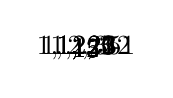
\begin{tikzpicture}
			\Tree
				[.\node{ \key{1,2,3}{5} };
					[.\node{ \key{1, 2, 3}{2} };
						[.\node{ \key{1, 2, 3}{-1} }; ]
						[.\node{ \key{1, 2}{2} };
							[.\node{ \key{1, 2}{0} }; ]
							[.\node{ \key{1}{2} }; ]
						]
					]
					[.\node{ \key{1, 2}{5} };
						[.\node{ \key{1, 2}{3} };
							[.\node{ \key{1, 2}{1} }; ]
							[.\node{ \key{1}{3} }; ]
						]
						[.\node{ \key{1}{5} };
							[.\node{ \key{1}{5} }; ]
							[.\node{ \key{1}{5} }; ]
						]
					]
				]
			\end{tikzpicture}
			\caption{}
			\label{fig:}
		\end{figure}
	}
	\item Suppose you are managing the construction of billboards on a highway of length $M$ miles. The possible sites for billboards are given by increasing mile numbers $x_{1}, x_{2}, \dots, x_{n}$ each in the interval $[0, M]$. If you place a billboard at location $x_{i}$, you receive a revenue of $r_{i} > 0$.\\\\Regulations require that \underline{no} two billboards be within less than or equal to 5 miles to each other. You'd like to place billboards at a subset of the sites so as to maximize your revenue, subject to this restriction.\\\\For example, suppose $M=20$, $n=4$, $\{ x_{1}, x_{2}, x_{3}, x_{4} \} = \{ 6, 7, 12, 14 \}$, $\{ r_{1}, r_{2}, r_{3}, r_{4} \} = \{ 5, 6, 5, 1 \}$. Then the optimal solution would be to place billboards at $x_{1}$ and $x_{3}$ for a total revenue of 10.\\\\Give an efficient algorithm that takes an instance of this problem as input and returns:
	\begin{enumerate}
	    \item the maximum total revenue that can be obtained from any valid subset of sites, and
		\item a subset of sites that achieves this maximum total revenue.
	\end{enumerate}
	\item Suppose that we have a set of $n$ activities, each with start time $s_{i}$ and finish time $f_{i}$, to schedule among a large number of lecture halls. We wish to schedule all the activities using as few lecture halls as possible. Give an efficient algorithm to determine which activity should use which lecture hall. Prove that your algorithm is optimal and discuss the asymptotic runtime of your algorithm. DO NOT JUST USE THE GREEDY-ALGORITHM ONCE PER ROOM; there is a more efficient algorithm.
\end{enumerate}
%</Recitation-9>

\end{document}